\chapter{System Testing and Verification}
\label{ch:system-testing}

This chapter introduces you to the testing setup and how we tested each module in isolation and the end-to-end integration that we planned and followed to prove to a high certainty the correctness of the system. \\

Testing of the project is done to check whether the actual results match what is expected, and ensure that each module is doing what it is intended to do, and to ensure that the system as a whole is working correctly. Our project depends on real world manuscript document image, so, most of our testing was done through testing the modules on different images, and checking whether the output is satisfactory compared to the results of similar projects. In the end, we test the workflow of the project to check whether the results are clear enough to interpret or not.

\section{Testing Setup}
\subsection{Setup Web Server}
Since the web server is build using Flask to accelerate the development of web application and the \acrfull{api}, we will install the flask framework and other libraries that depends on it in this section. Also we will setup machine learning environment for predicting the manuscript image.

\subsubsection{Installing Required Libraries}
Run the following:
\begin{verbatim}
$ python --version
\end{verbatim}
If it's 3.x, you are good to go with installing the other libraries. The libraries is grouped into a text file to install all of them once by one command. The file requirements.txt file will include the following content:

\begin{verbatim}
apispec==5.1.1
apispec_webframeworks==0.5.2
Flask==2.0.2
Flask_Login==0.5.0
flask_swagger_ui==3.36.0
marshmallow==3.15.0
numpy==1.21.4
opencv_python==4.5.4.58
pandas==1.1.4
SQLAlchemy==1.4.27
tensorflow==2.7.0
tensorflow_addons==0.16.1
Werkzeug==2.0.0
gunicorn==20.1.0
\end{verbatim}

\noindent
Once you copied and created this text file, run the following:

\begin{verbatim}
$ pip install -r requirements.txt
\end{verbatim}

\subsubsection{Start Script}
After installing all required libraries, run the following script to start flask app to start web application and the API.

\begin{verbatim}
$ python -m flask run
\end{verbatim}

\subsection{Setup Mobile Application}
The mobile application is built using the great flutter framework launched by Google which gives us the flexibility to create applications that work on Android and iOS operating systems.
In this section, we will explain the steps that we will follow to download and install the packages and run the application.
\subsubsection{Installing Required Libraries}
To install the packages needed to run the application, we go to the pubspec.yaml file located in the root of the application filesand make sure that the following packages are correctly present:
\begin{verbatim}
cupertino_icons: ^1.0.2
provider: ^6.0.3
shared_preferences: ^2.0.12
flutter_svg: ^1.0.3
easy_localization: ^3.0.0
image_picker: ^0.8.4+11
image_cropper: ^1.5.0
dio: any
path_provider: ^2.0.9
rxdart: ^0.27.3
\end{verbatim}
then run the following:
\begin{verbatim}
$ flutter pub get
\end{verbatim}

\subsubsection{Start Script}
After installing all required libraries, run the following command in the terminal to start flutter app.

\begin{verbatim}
$ flutter run lib/main.dart
\end{verbatim}

\section{Testing Plan and Strategy}
Our main goal in evaluating each module in ASAR was to make sure it met all functional and non-functional requirements that were specified earlier. Testing is almost as challenging as development.

\subsection{Module Testing}
We follow a separate module testing to test ASAR. For each module, we take the output of previous module and test the output resulted form the module. We take one sample image shown in figure \ref{fig:real-world-sample} to forward test each module on it separately.

\begin{figure}[H]
    \centering
    \includegraphics[width=6cm, height=9cm]{images/line_step1.png}
    \caption{Test real world manuscript image}
    \label{fig:real-world-sample}
\end{figure}

\subsubsection{Line Segmentation Testing}

We implemented this module using computer vision preprocessing techniques explain in details in chapter 3. The line segmentation is done by applied some preprocessing in order to prepare it for morphological operations like Gray scale, Binary thresholding, Gaussian blur, and Gaussian thresholding. Then, morphological operators like erosion, dilation, opening and closing are applied and shown in figure
\ref{fig:line_segmentation}.

\begin{figure}[H]
     \centering%
    %  \begin{subfigure}[b]{0.3\textwidth}
    %      \centering
    %      \includegraphics[width=\textwidth]{images/line_step1.png}
    %      \caption{Original Image}
    %      \label{fig:test_Original}
    %  \end{subfigure}
    %  \hfill%
     \begin{subfigure}[b]{0.3\textwidth}
         \centering
         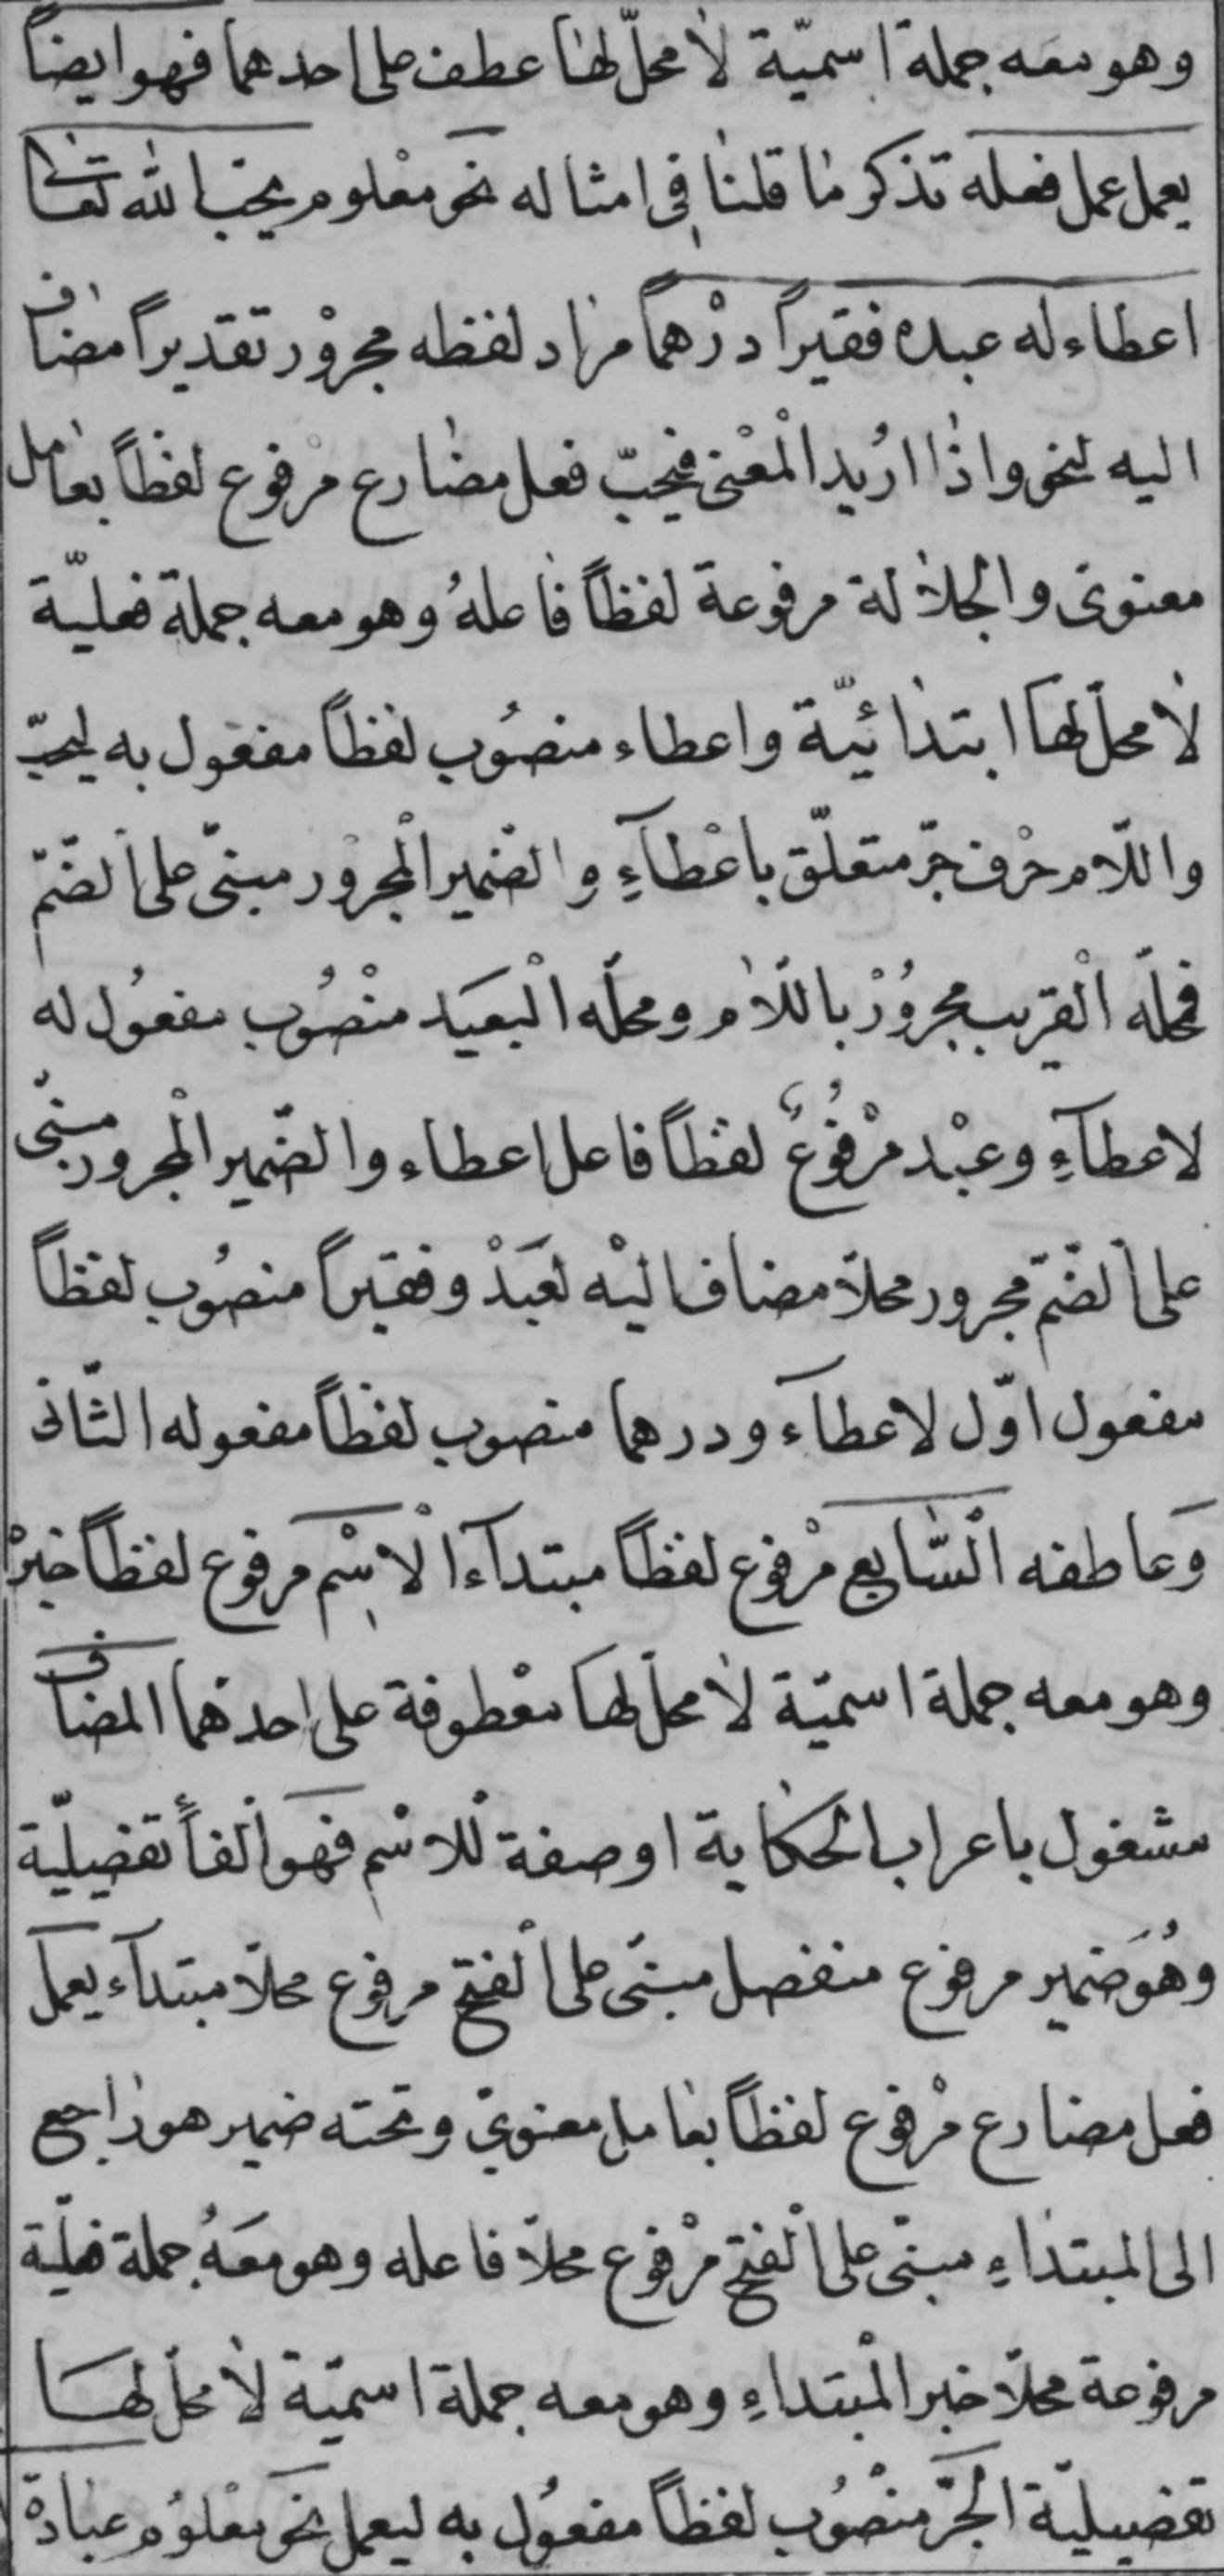
\includegraphics[width=\textwidth, height=8cm]{images/line_step2.jpg}
         \caption{Gray Scale Image}
         \label{fig:test_Gray_Scale}
     \end{subfigure}
     \hfill
      \begin{subfigure}[b]{0.3\textwidth}
         \centering
         
\includegraphics[width=\textwidth, height=8cm]{images/line_step3.png}
         \caption{Binary Inverted Image}
         \label{fig:test_Binary}
     \end{subfigure}
     \hfill%
      \begin{subfigure}[b]{0.3\textwidth}
         \centering
         
\includegraphics[width=\textwidth, height=8cm]{images/line_step4.png}
         \caption{Closing Image}
         \label{fig:test_Closing}
     \end{subfigure}
     \hfill%
      \begin{subfigure}[b]{0.3\textwidth}
         \centering
         
\includegraphics[width=\textwidth, height=8cm]{images/line_step5.png}
         \caption{Erode Image}
         \label{fig:test_Erode}
     \end{subfigure}
     \hfill%
      \begin{subfigure}[b]{0.3\textwidth}
         \centering
         
\includegraphics[width=\textwidth, height=8cm]{images/line_step6.png}
         \caption{Threshold Image}
         \label{fig:test_Threshold}
     \end{subfigure}
     \hfill%
      \begin{subfigure}[b]{0.3\textwidth}
         \centering
         
\includegraphics[width=\textwidth, height=8cm]{images/line_step7.png}
         \caption{Dilated Image}
         \label{fig:test_Dilated}
     \end{subfigure}

        \caption{Morphological operations for line segmentation.}
        \label{fig:line_segmentation}
\end{figure}


After preparing the image by morphological operations, then, contours are drawn based on dilation and threshold to select the largest contours area as a separately line from the image. Figure \ref{fig:line-segmentation-results} shows the result lines based on contours area.

\begin{figure}[H]
     \centering%
     \begin{subfigure}[b]{0.3\textwidth}
         \centering
         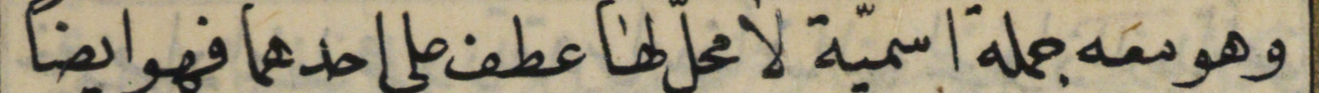
\includegraphics[width=\textwidth]{images/lines/_1.png}
         \caption{Line 1}
     \end{subfigure}
     \hfill%
     \begin{subfigure}[b]{0.3\textwidth}
         \centering
         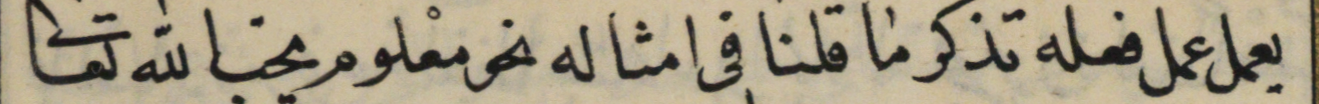
\includegraphics[width=\textwidth]{images/lines/_2.png}
         \caption{Line 2}
     \end{subfigure}
     \hfill%
     \begin{subfigure}[b]{0.3\textwidth}
         \centering
         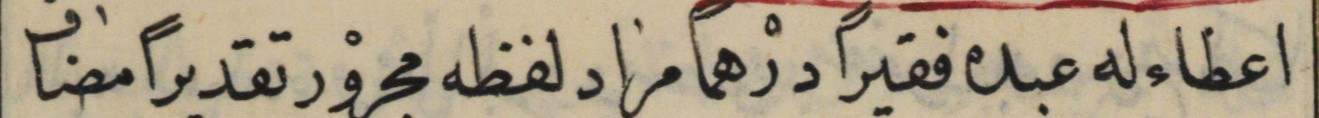
\includegraphics[width=\textwidth]{images/lines/_3.png}
         \caption{Line 3}
     \end{subfigure}
     \hfill%
     \begin{subfigure}[b]{0.3\textwidth}
         \centering
         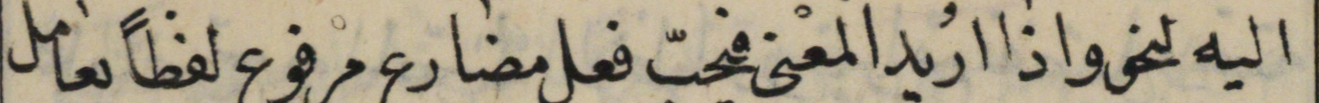
\includegraphics[width=\textwidth]{images/lines/_4.png}
         \caption{Line 4}
     \end{subfigure}
     \hfill%
     \begin{subfigure}[b]{0.3\textwidth}
         \centering
         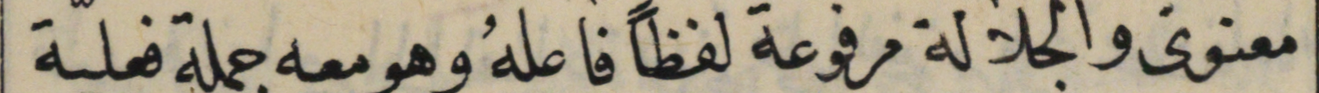
\includegraphics[width=\textwidth]{images/lines/_5.png}
         \caption{Line 5}
     \end{subfigure}
     \hfill%
     \begin{subfigure}[b]{0.3\textwidth}
         \centering
         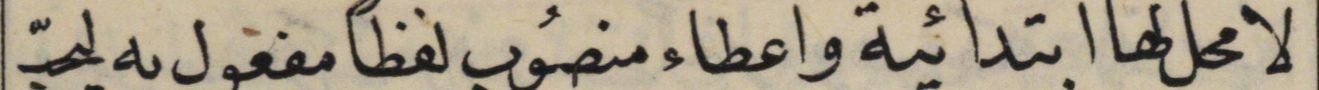
\includegraphics[width=\textwidth]{images/lines/_6.png}
         \caption{Line 6}
     \end{subfigure}
     \hfill%
     \begin{subfigure}[b]{0.3\textwidth}
         \centering
         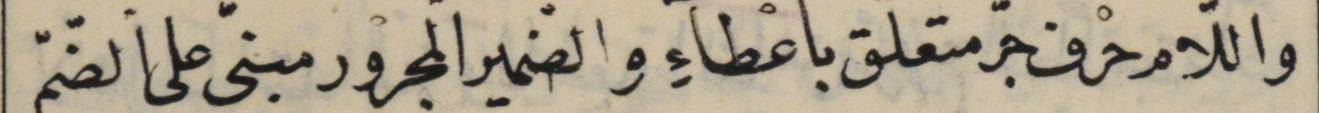
\includegraphics[width=\textwidth]{images/lines/_7.png}
         \caption{Line 7}
     \end{subfigure}
     \hfill%
     \begin{subfigure}[b]{0.3\textwidth}
         \centering
         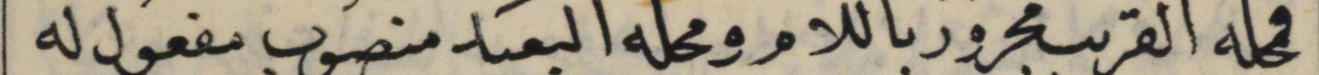
\includegraphics[width=\textwidth]{images/lines/_8.png}
         \caption{Line 8}
     \end{subfigure}
     \hfill%
     \begin{subfigure}[b]{0.3\textwidth}
         \centering
         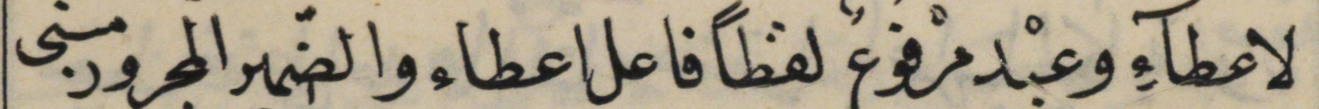
\includegraphics[width=\textwidth]{images/lines/_9.png}
         \caption{Line 9}
     \end{subfigure}
     \hfill%
     \begin{subfigure}[b]{0.3\textwidth}
         \centering
         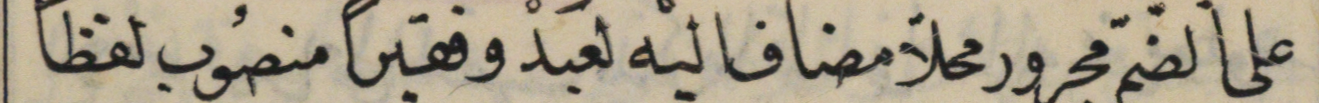
\includegraphics[width=\textwidth]{images/lines/_10.png}
         \caption{Line 10}
     \end{subfigure}
     \hfill%
     \begin{subfigure}[b]{0.3\textwidth}
         \centering
         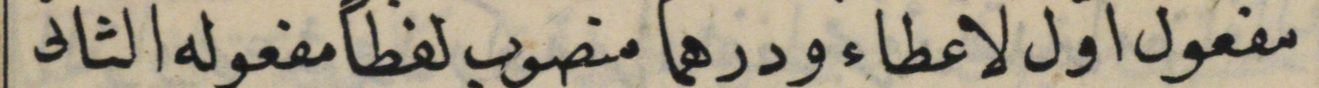
\includegraphics[width=\textwidth]{images/lines/_11.png}
         \caption{Line 11}
     \end{subfigure}
     \hfill%
     \begin{subfigure}[b]{0.3\textwidth}
         \centering
         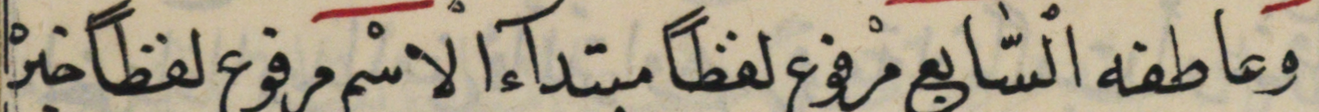
\includegraphics[width=\textwidth]{images/lines/_12.png}
         \caption{Line 12}
     \end{subfigure}
     \hfill%
     \begin{subfigure}[b]{0.3\textwidth}
         \centering
         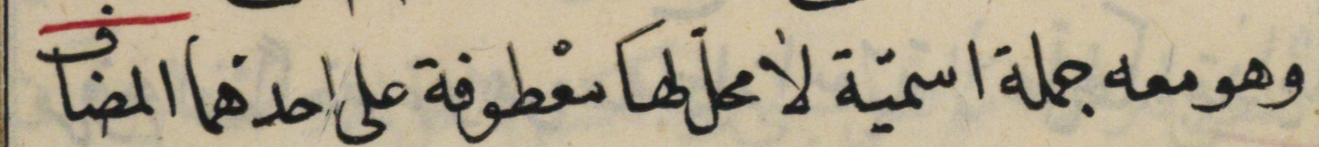
\includegraphics[width=\textwidth]{images/lines/_13.png}
         \caption{Line 13}
     \end{subfigure}
     \hfill%
     \begin{subfigure}[b]{0.3\textwidth}
         \centering
         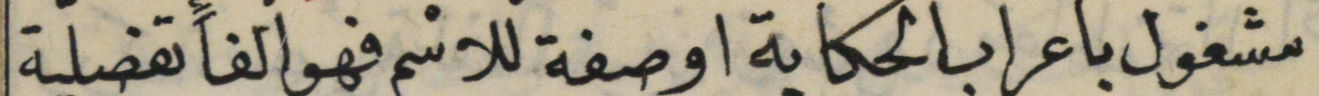
\includegraphics[width=\textwidth]{images/lines/_14.png}
         \caption{Line 14}
     \end{subfigure}
     \hfill%
     \begin{subfigure}[b]{0.3\textwidth}
         \centering
         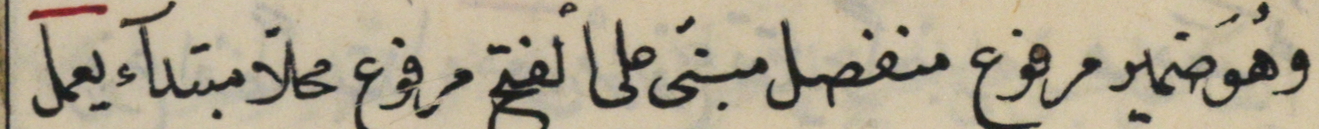
\includegraphics[width=\textwidth]{images/lines/_15.png}
         \caption{Line 15}
     \end{subfigure}
     \hfill%
     \begin{subfigure}[b]{0.3\textwidth}
         \centering
         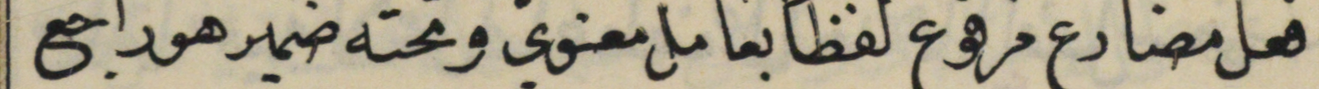
\includegraphics[width=\textwidth]{images/lines/_16.png}
         \caption{Line 16}
     \end{subfigure}
     \hfill%
     \begin{subfigure}[b]{0.3\textwidth}
         \centering
         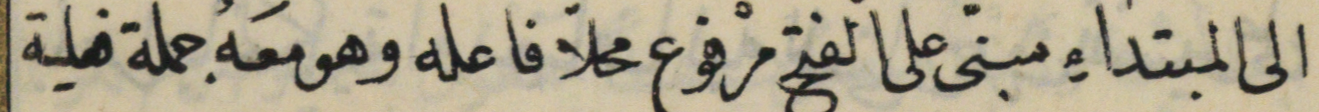
\includegraphics[width=\textwidth]{images/lines/_17.png}
         \caption{Line 17}
     \end{subfigure}
     \hfill%
     \begin{subfigure}[b]{0.3\textwidth}
         \centering
         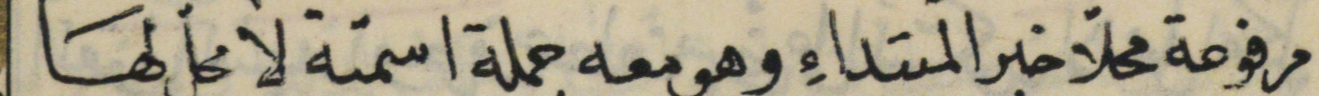
\includegraphics[width=\textwidth]{images/lines/_18.png}
         \caption{Line 18}
     \end{subfigure}
     \hfill%
     \begin{subfigure}[b]{0.3\textwidth}
         \centering
         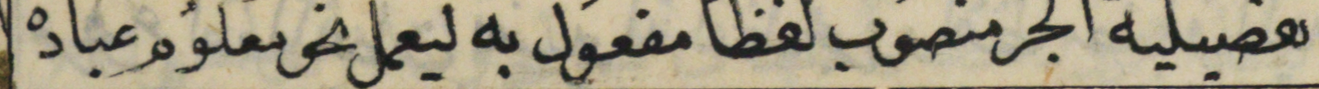
\includegraphics[width=\textwidth]{images/lines/_19.png}
         \caption{Line 19}
     \end{subfigure}
    \caption{Output of line segmentation module.}
    \label{fig:line-segmentation-results}
\end{figure}


\subsubsection{Word Segmentation Testing}
We implemented this module using computer vision preprocessing and find contours techniques explain in details in chapter 3.The word segmentation is done by applied some preprocessing such as Gray-Scale, Thresholding and Remove dots on each individual line that extracted from a lines segmentation step in order to prepare it for Finding Contours technique and shown in figure.
\begin{figure}[H]
     \centering%
     \begin{subfigure}[b]{0.3\textwidth}
         \centering
         \includegraphics[width=\textwidth, height=9cm]{images/pre_word/word (1).png}
         \caption{Gray Scale}
         \label{fig:test-word_Gray_Scale}
     \end{subfigure}
     \hfill
      \begin{subfigure}[b]{0.3\textwidth}
         \centering
         
\includegraphics[width=\textwidth, height=9cm]{images/pre_word/word2.png}
         \caption{Binary Threshold}
         \label{fig:test-word_Binary}
     \end{subfigure}
     \hfill%
      \begin{subfigure}[b]{0.3\textwidth}
         \centering
         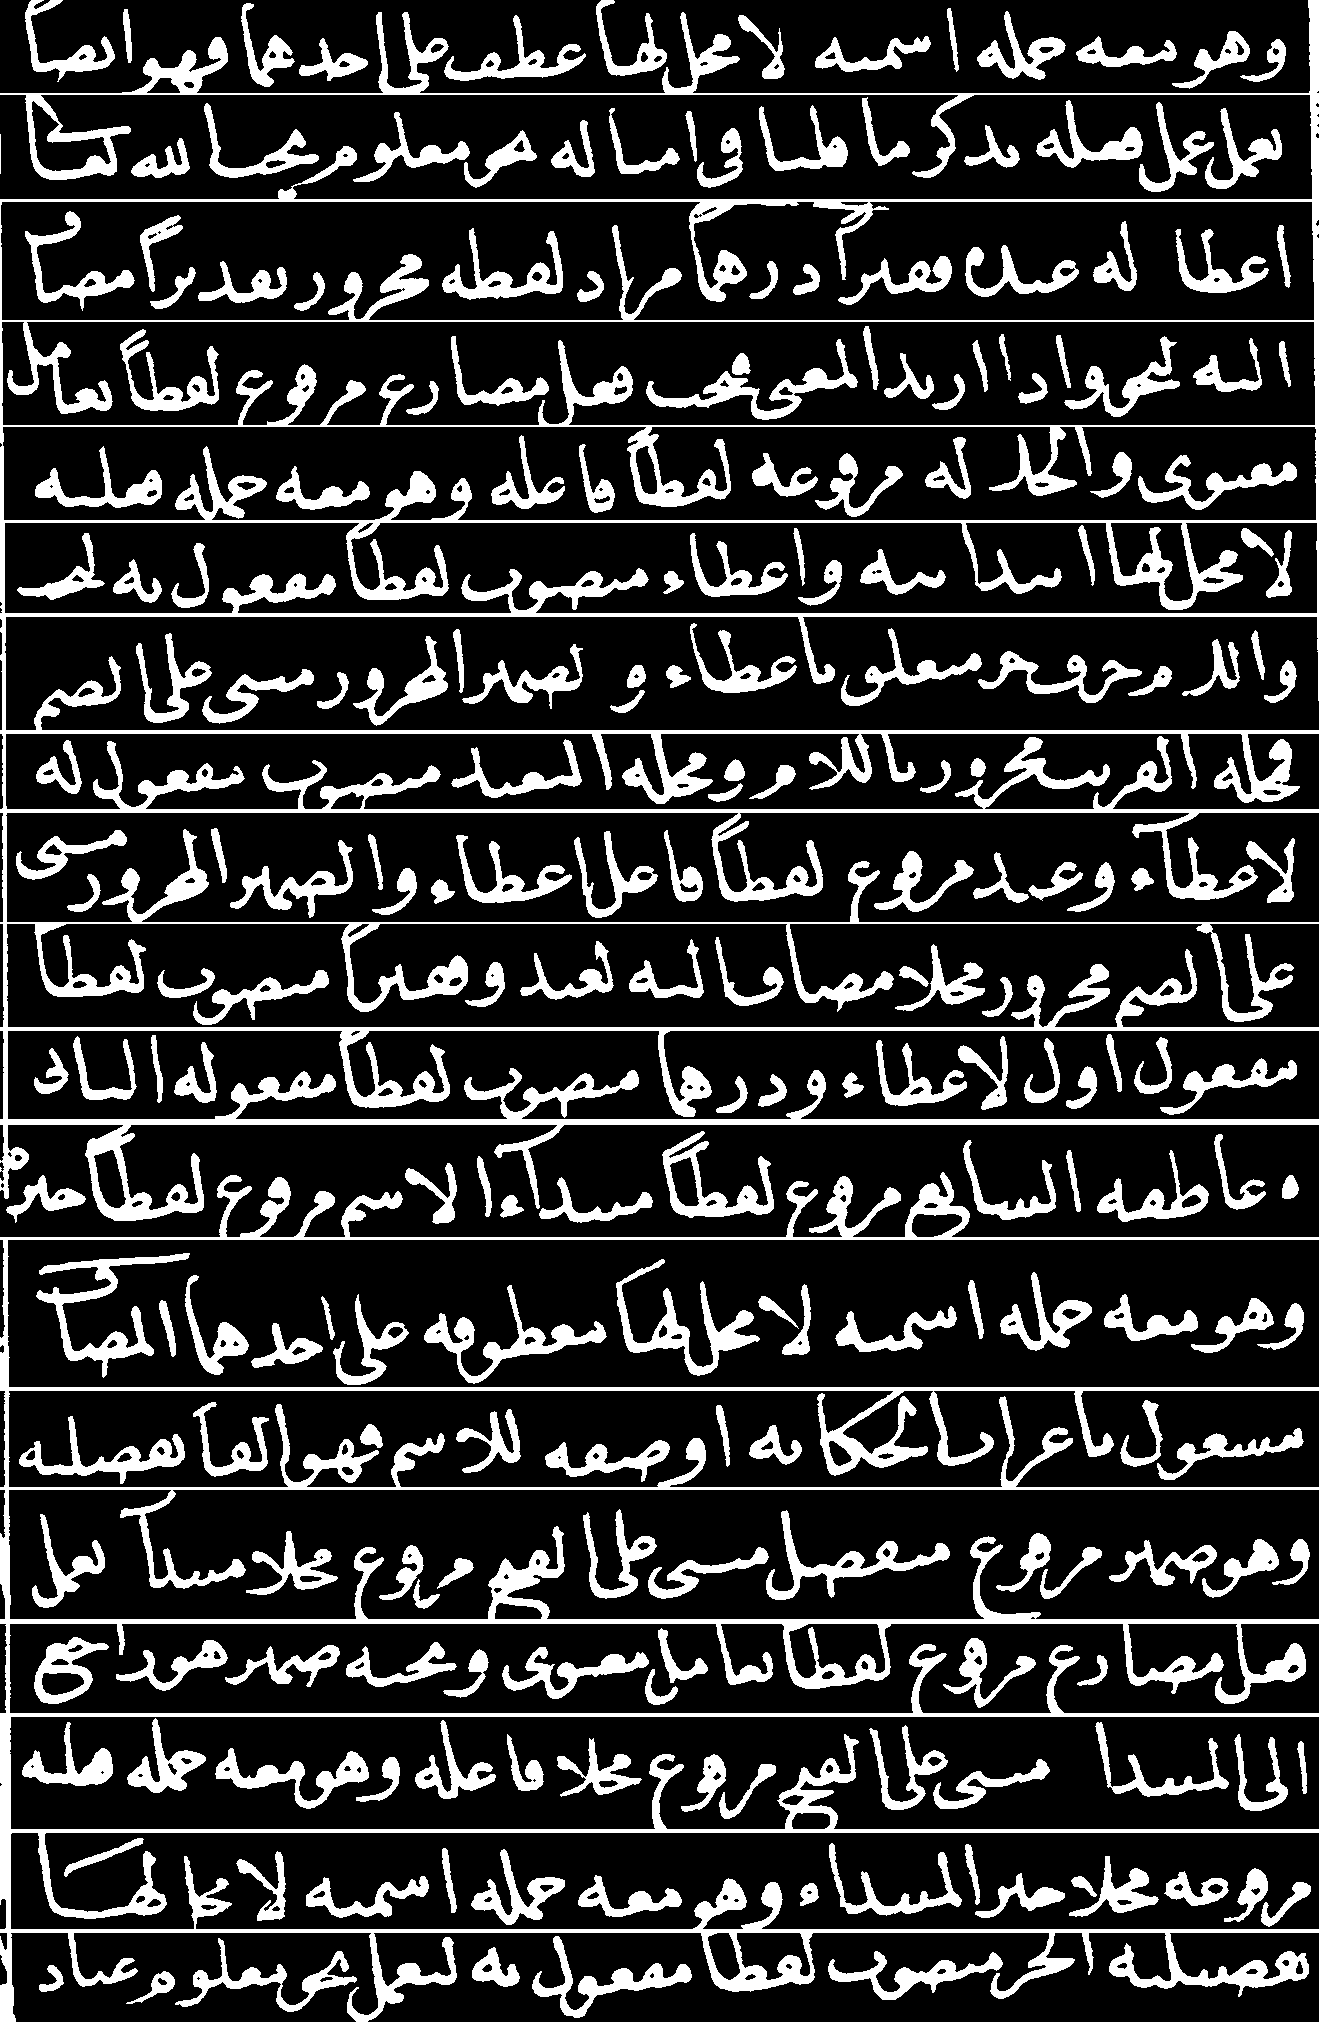
\includegraphics[width=\textwidth, height=9cm]{images/pre_word/word3.png}
         \caption{Removing Dots}
         \label{fig:test_Removing-Dots}
     \end{subfigure}

        \caption{preprocessing After Word Segmentation.}
        \label{fig:pre-word_segmentation}
\end{figure}

After preparing all lines by some preprocessing, then contours are drawn on each individual line and cropped all these contours to extract all sub-words from each line.Figure  shows the result sub-words for all lines.
\begin{figure}[H]
     \centering%
     \begin{subfigure}[b]{0.3\textwidth}
         \centering
         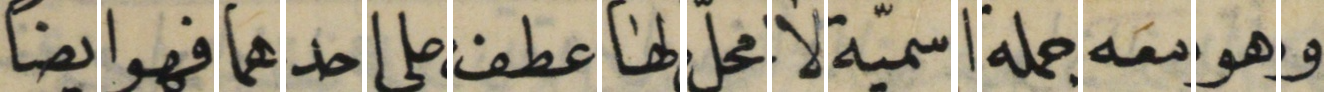
\includegraphics[width=\textwidth]{images/word-seg/line-1.png}
         \caption{Sub-words of Line 1}
     \end{subfigure}
     \centering%
     \begin{subfigure}[b]{0.3\textwidth}
         \centering
         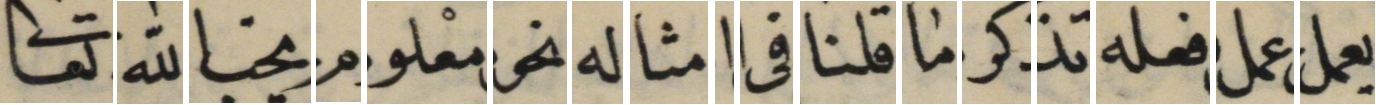
\includegraphics[width=\textwidth]{images/word-seg/line-2.png}
         \caption{Sub-words of Line 2}
     \end{subfigure}
     \centering%
     \begin{subfigure}[b]{0.3\textwidth}
         \centering
         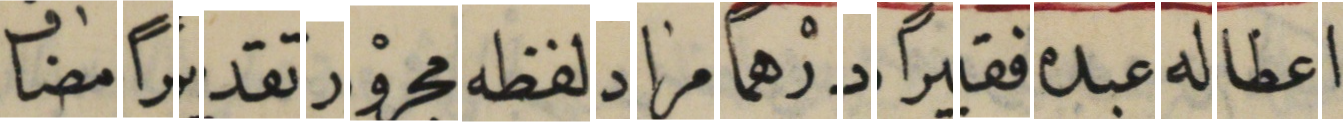
\includegraphics[width=\textwidth]{images/word-seg/line-3.png}
         \caption{Sub-words of Line 3}
     \end{subfigure}
     \centering%
     \begin{subfigure}[b]{0.3\textwidth}
         \centering
         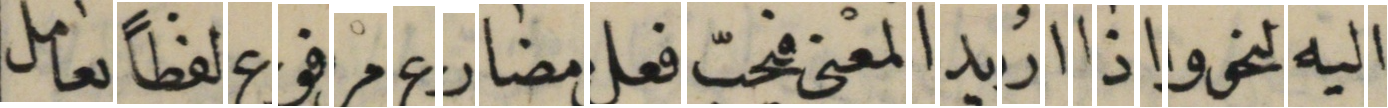
\includegraphics[width=\textwidth]{images/word-seg/line-4.png}
         \caption{Sub-words of Line 4}
     \end{subfigure}
     \centering%
     \begin{subfigure}[b]{0.3\textwidth}
         \centering
         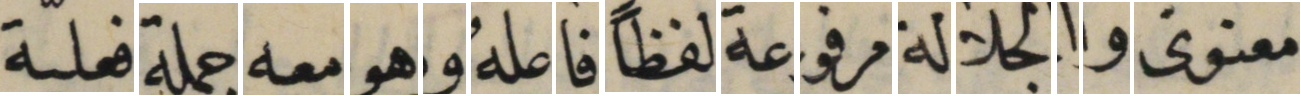
\includegraphics[width=\textwidth]{images/word-seg/line-5.png}
         \caption{Sub-words of Line 5}
     \end{subfigure}
     \centering%
     \begin{subfigure}[b]{0.3\textwidth}
         \centering
         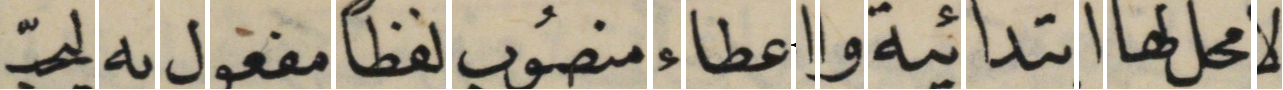
\includegraphics[width=\textwidth]{images/word-seg/line-6.png}
         \caption{Sub-words of Line 6}
     \end{subfigure}
     \centering%
     \begin{subfigure}[b]{0.3\textwidth}
         \centering
         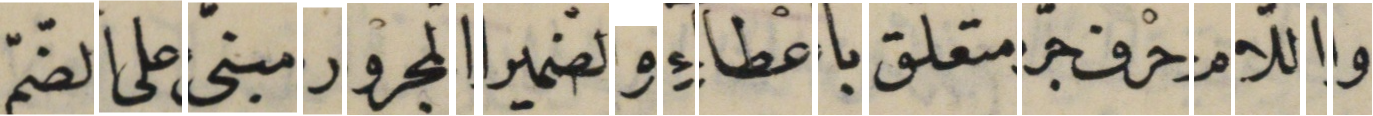
\includegraphics[width=\textwidth]{images/word-seg/line-7.png}
         \caption{Sub-words of Line 7}
     \end{subfigure}
     \centering%
     \begin{subfigure}[b]{0.3\textwidth}
         \centering
         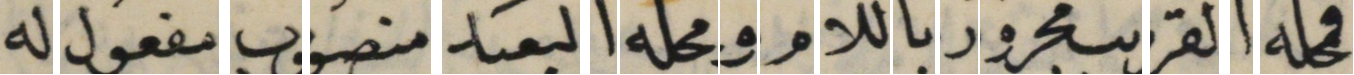
\includegraphics[width=\textwidth]{images/word-seg/line-8.png}
         \caption{Sub-words of Line 8}
     \end{subfigure}
     \centering%
     \begin{subfigure}[b]{0.3\textwidth}
         \centering
         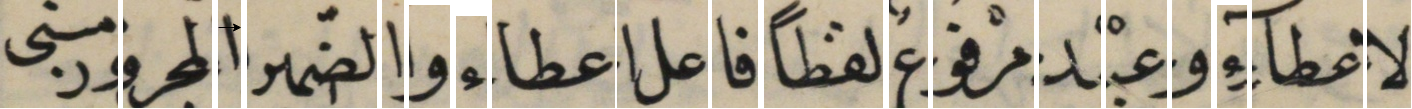
\includegraphics[width=\textwidth]{images/word-seg/line-9.png}
         \caption{Sub-words of Line 9}
     \end{subfigure}
     \centering%
     \begin{subfigure}[b]{0.3\textwidth}
         \centering
         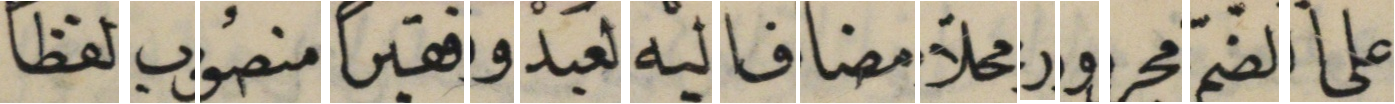
\includegraphics[width=\textwidth]{images/word-seg/line-10.png}
         \caption{Sub-words of Line 10}
     \end{subfigure}
     \centering%
     \begin{subfigure}[b]{0.3\textwidth}
         \centering
         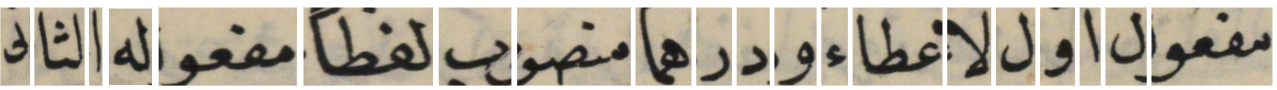
\includegraphics[width=\textwidth]{images/word-seg/line-11.png}
         \caption{Sub-words of Line 11}
     \end{subfigure}
     \centering%
     \begin{subfigure}[b]{0.3\textwidth}
         \centering
         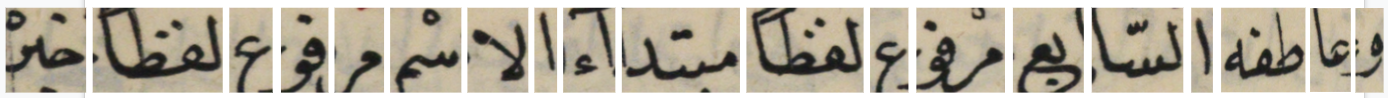
\includegraphics[width=\textwidth]{images/word-seg/line-12.png}
         \caption{Sub-words of Line 12}
     \end{subfigure}
     \centering%
     \begin{subfigure}[b]{0.3\textwidth}
         \centering
         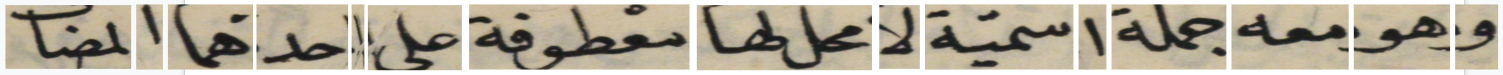
\includegraphics[width=\textwidth]{images/word-seg/line-13.png}
         \caption{Sub-words of Line 13}
     \end{subfigure}
     \centering%
     \begin{subfigure}[b]{0.3\textwidth}
         \centering
         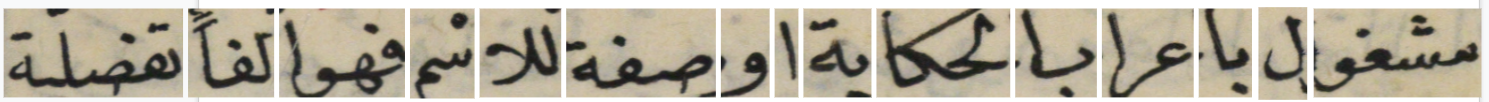
\includegraphics[width=\textwidth]{images/word-seg/line-14.png}
         \caption{Sub-words of Line 14}
     \end{subfigure}
     \centering%
     \begin{subfigure}[b]{0.3\textwidth}
         \centering
         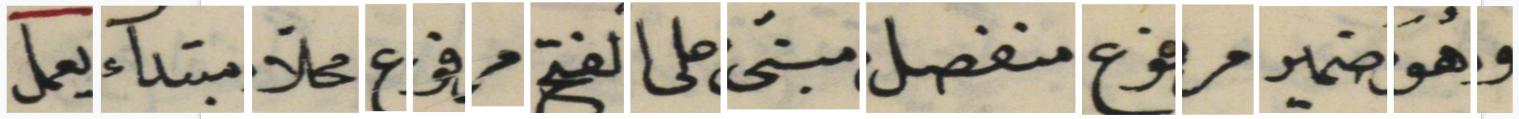
\includegraphics[width=\textwidth]{images/word-seg/line-15.png}
         \caption{Sub-words of Line 15}
     \end{subfigure}
     \centering%
     \begin{subfigure}[b]{0.3\textwidth}
         \centering
         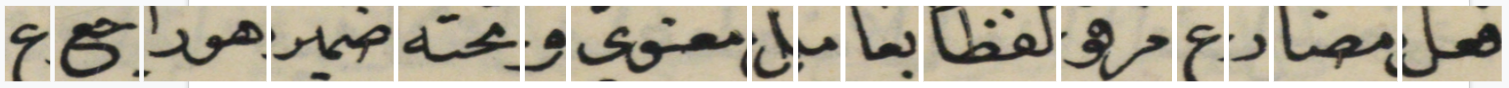
\includegraphics[width=\textwidth]{images/word-seg/line-16.png}
         \caption{Sub-words of Line 16}
     \end{subfigure}
     \centering%
     \begin{subfigure}[b]{0.3\textwidth}
         \centering
         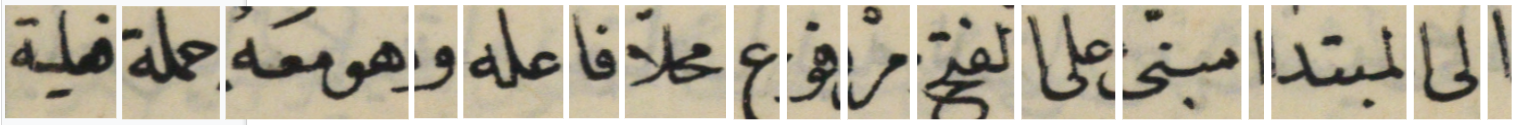
\includegraphics[width=\textwidth]{images/word-seg/line-17.png}
         \caption{Sub-words of Line 17}
     \end{subfigure}
     \centering%
     \begin{subfigure}[b]{0.3\textwidth}
         \centering
         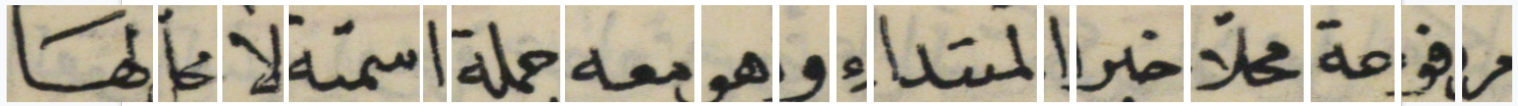
\includegraphics[width=\textwidth]{images/word-seg/line-18.png}
         \caption{Sub-words of Line 18}
     \end{subfigure}
     \centering%
     \begin{subfigure}[b]{0.3\textwidth}
         \centering
         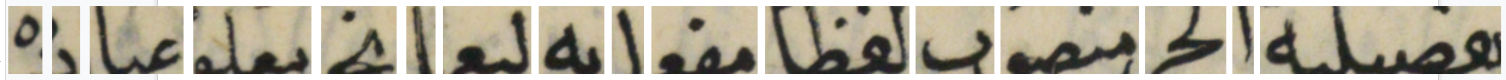
\includegraphics[width=\textwidth]{images/word-seg/line-19.png}
         \caption{Sub-words of Line 19}
     \end{subfigure}
    \caption{Output of word segmentation module.}
    \label{fig:line-segmentation-results}
\end{figure}
fig
\subsubsection{Model Testing}
The PHOSC model takes a lot of time for training, depending the capacity of the GPU and its edition. We have used azure cloud service with compute consist of a K-Tesla GPU with memory size 56GB and 380GB disk storage in the training and testing. Since this machine is costly, we did training the model with 50 epochs with average of 3 days on the specific GPU. \\

After training the model on 187,913 samples, we evaluated them on a separate test of manuscript images. The summary of our results is presented as follows. Figure \ref{fig:training-graphs} showing the training process of our model which choose cosine similarity as performance metric to measure how well the classifier performs against the training and validation data.

\begin{figure}[H]
    \centering
    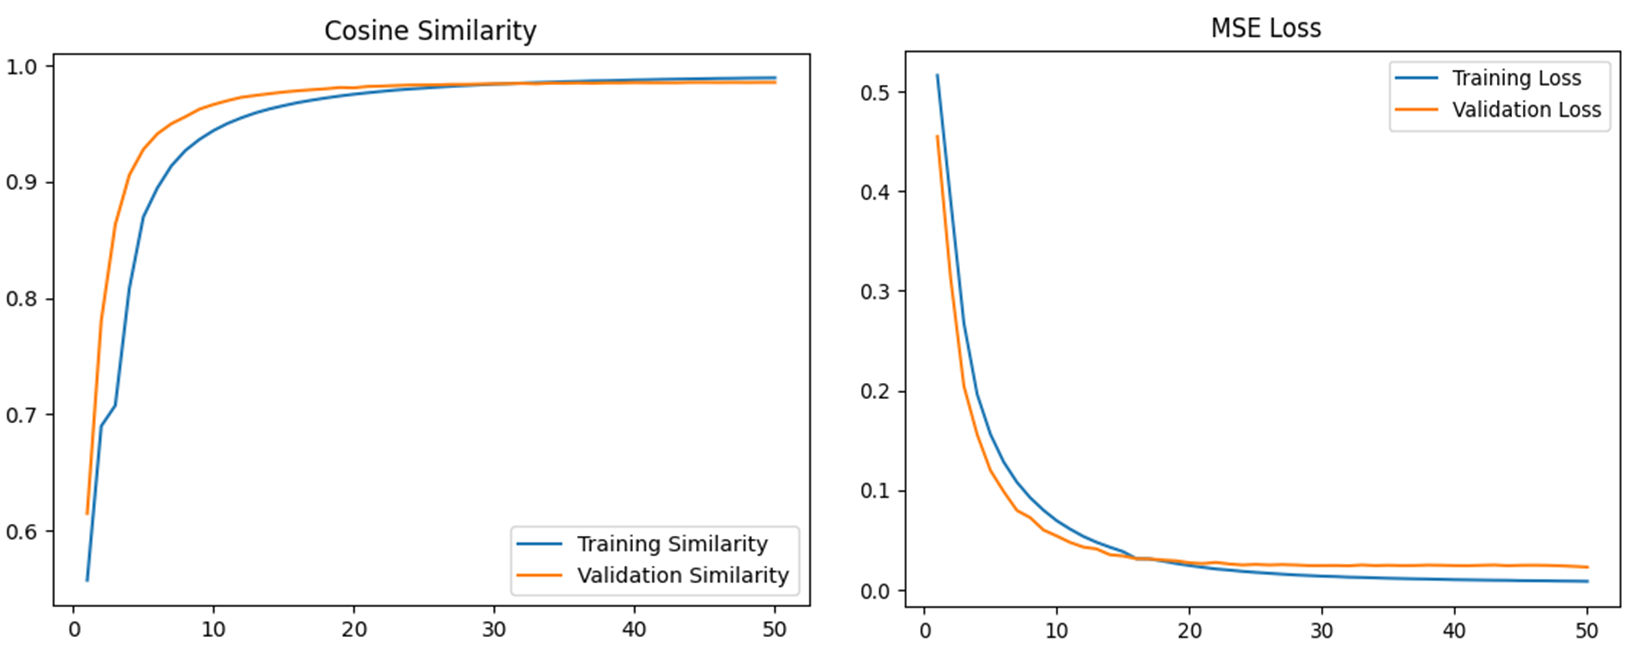
\includegraphics[width=15cm]{images/training-graphs.png}
    \caption{Training graphs showing the cosine similarity and loss against number of epochs}
    \label{fig:training-graphs}
\end{figure}

For testing, Figure \ref{fig:confusion-matrix} presents the confusion matrix for predictions on our test set (15,592 samples). The confusion matrix has been computed between words of different lengths to uncover any biases of the model (if any). It is difficult to visualize the class specific confusion matrix as there are over 5,429 word labels with very few (often only 1) images per word label. The length of the predicted word labels is mostly within a range of the length of the true word label. In general, the model is not biased towards words of any specific length. The high values along the diagonal indicates that the model is often predicting the word of the correct length.

\begin{figure}[H]
    \centering
    \includegraphics[width=12cm]{images/confusion-matrix.png}
    \caption{Confusion matrix (normalized) for the predicted word length}
    \label{fig:confusion-matrix}
\end{figure}

Figure \ref{fig:test-accuracy} showing the accuracy based on corrected predictions for world length which achieved 92\% for unseen words.

\begin{figure}[H]
    \centering
    \includegraphics[width=12cm]{images/test-accuracy.png}
    \caption{Testing accuracy based on the predicted word length}
    \label{fig:test-accuracy}
\end{figure}

\subsection{Integration Testing}
After merging all our modules together and testing the whole project integrated, we noticed that the final results are highly dependent on three things. First is the image quality and if the images are not clear and taken with a bad camera which effect on the correct predictions. Second is the segmentation accuracy with highly Arabic connected multiple words with each which the model is not accurate to deal with multiple words which the results too are not the best. Third thing is the hardware and amount of dataset are limited to train the PHOSC model in order to fit in all Arabic manuscripts challenges. A fast GPU with large memory size would be of a huge advantage.